\documentclass[12pt]{article}

\usepackage{tikz}
\usetikzlibrary{automata, positioning, arrows}

\tikzset{
    ->, >=stealth,
    node distance=2.2cm,
    every state/.style={thick, fill=gray!10},
}

\usepackage{amsmath}
\usepackage{amssymb}
\usepackage{enumitem}
\usepackage{geometry}
\geometry{margin=2.5cm}

\title{Máquinas de Turing para Três Linguagens: A, B e C}
\date{}

\begin{document}

\maketitle

\section{Introdução}

Este documento apresenta três Máquinas de Turing completas para as linguagens abaixo, todas definidas sobre o alfabeto $\Sigma = \{0, 1\}$:

\begin{itemize}
    \item Linguagem A: $\#0(w) = \#1(w)$
    \item Linguagem B: $\#0(w) = 2 \cdot \#1(w)$
    \item Linguagem C: complemento de B
\end{itemize}

Incluímos:
\begin{itemize}
    \item Definições formais
    \item Máquinas de Turing completas
    \item Diagramas formais em TikZ
    \item Tabelas de transição
\end{itemize}

\newpage

% ============================================================
\section{Linguagem A}

\subsection{Definição}

\[
A = \{ w \in \{0,1\}^* \mid \#0(w) = \#1(w) \}
\]

A ideia da MT é emparelhar zeros e uns usando marcações:
\begin{itemize}
    \item $0 \to X$
    \item $1 \to Y$
\end{itemize}

Cada símbolo deve encontrar um par.

\subsection{Diagrama de Estados (TikZ)}

\begin{center}
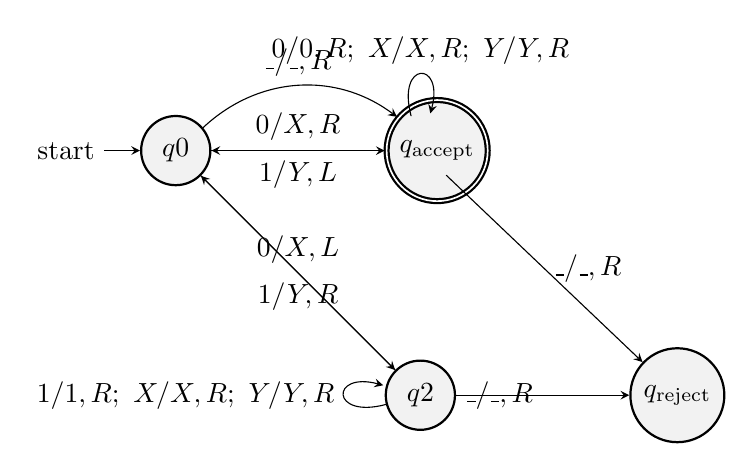
\begin{tikzpicture}

\node[state, initial] (q0) {$q0$};
\node[state] (q1) [right=of q0] {$q1$};
\node[state] (q2) [below=of q1] {$q2$};
\node[state] (qr) [right=of q2] {$q_{\text{reject}}$};
\node[state, accepting] (qa) [right=of q0] {$q_{\text{accept}}$};

\draw (q0) edge[above] node{$0/X,R$} (q1);
\draw (q0) edge[below] node{$1/Y,R$} (q2);
\draw (q0) edge[bend left=40, above] node{$\_/ \_,R$} (qa);

\draw (q1) edge[loop above] node{$0/0,R;\ X/X,R;\ Y/Y,R$} ();
\draw (q1) edge[below] node{$1/Y,L$} (q0);
\draw (q1) edge[right] node{$\_/ \_,R$} (qr);

\draw (q2) edge[loop left] node{$1/1,R;\ X/X,R;\ Y/Y,R$} ();
\draw (q2) edge[above] node{$0/X,L$} (q0);
\draw (q2) edge[left] node{$\_/ \_,R$} (qr);

\end{tikzpicture}
\end{center}


\newpage

% ============================================================
\section{Linguagem B}

\subsection{Definição}

\[
B = \{ w \in \{0,1\}^* \mid \#0(w) = 2 \cdot \#1(w) \}
\]

Condições:
\begin{itemize}
    \item Cada símbolo `1` deve ter \textbf{dois zeros} associados.
    \item Se não houver uns, a string só é aceita se não houver zeros.
    \item A máquina marca:
    \[
    1 \to A,\quad 0 \to B
    \]
\end{itemize}

\subsection{Descrição da MT}

\begin{enumerate}
    \item Em $q0$, encontrar um `1` não marcado.
    \item Marcar como $A$.
    \item Em $q2$, procurar o primeiro zero.
    \item Em $q3$, procurar o segundo zero.
    \item Em $q4$, retornar ao início.
    \item Em $q5$, verificar sobras.
\end{enumerate}

\subsection{Diagrama da MT B}

\begin{center}
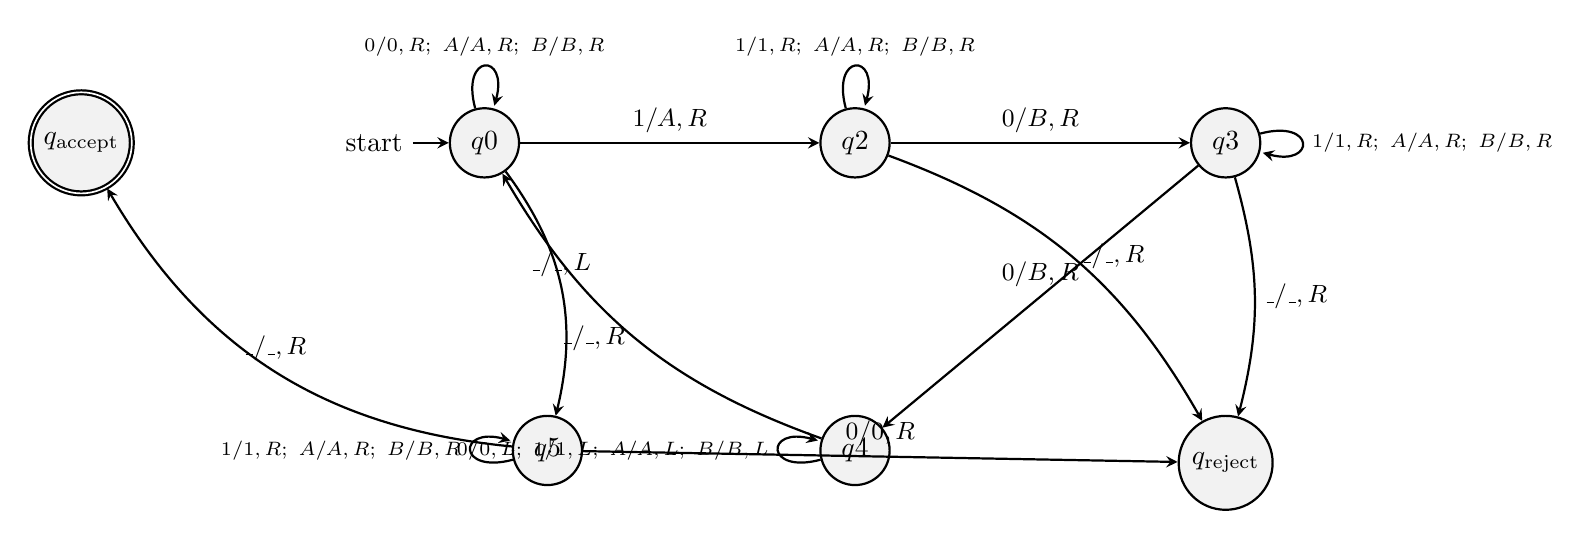
\begin{tikzpicture}[node distance=3.8cm,>=stealth,->,thick]

\node[state, initial] (q0) {$q0$};
\node[state] (q2) [right=of q0] {$q2$};
\node[state] (q3) [right=of q2] {$q3$};

\node[state] (q4) [below=3cm of q2] {$q4$};
\node[state] (q5) [left=3cm of q4] {$q5$};

\node[state, accepting] (qa) [left=4cm of q0] {$q_{\text{accept}}$};
\node[state] (qr) [below=3cm of q3] {$q_{\text{reject}}$};

% q0
\draw (q0) edge[above] node[font=\small] {$1/A,R$} (q2);
\draw (q0) edge[loop above] node[font=\scriptsize] {$0/0,R;\ A/A,R;\ B/B,R$} ();
\draw (q0) edge[bend left=25, above] node[font=\small] {$\_/\_,L$} (q5);

% q2
\draw (q2) edge[above] node[font=\small] {$0/B,R$} (q3);
\draw (q2) edge[loop above] node[font=\scriptsize] {$1/1,R;\ A/A,R;\ B/B,R$} ();
\draw (q2) edge[bend left=20, right] node[font=\small] {$\_/\_,R$} (qr);

% q3
\draw (q3) edge[above] node[font=\small] {$0/B,R$} (q4);
\draw (q3) edge[loop right] node[font=\scriptsize] {$1/1,R;\ A/A,R;\ B/B,R$} ();
\draw (q3) edge[bend left=15, right] node[font=\small] {$\_/\_,R$} (qr);

% q4
\draw (q4) edge[loop left] node[font=\scriptsize] {$0/0,L;\ 1/1,L;\ A/A,L;\ B/B,L$} ();
\draw (q4) edge[bend left=20, left] node[font=\small] {$\_/\_,R$} (q0);

% q5
\draw (q5) edge[above] node[font=\small] {$0/0,R$} (qr);
\draw (q5) edge[loop left] node[font=\scriptsize] {$1/1,R;\ A/A,R;\ B/B,R$} ();
\draw (q5) edge[bend left=27, above] node[font=\small] {$\_/\_,R$} (qa);

\end{tikzpicture}
\end{center}


\newpage

% ============================================================
\section{Linguagem C}

\subsection{Definição}

\[
C = \overline{B} = \{ w \mid \#0(w) \neq 2 \cdot \#1(w) \}
\]

\subsection{Construção da MT C}

Como B é uma \textbf{máquina decisora}, podemos tomar seu complemento:

\begin{itemize}
    \item C simula B.
    \item Se B aceita, C rejeita.
    \item Se B rejeita, C aceita.
\end{itemize}

Introduzimos:
\begin{itemize}
    \item $q_{\text{start}}$
    \item $q_{C\_accept}$
    \item $q_{C\_reject}$
\end{itemize}

\subsection{Diagrama da MT C}

\begin{center}
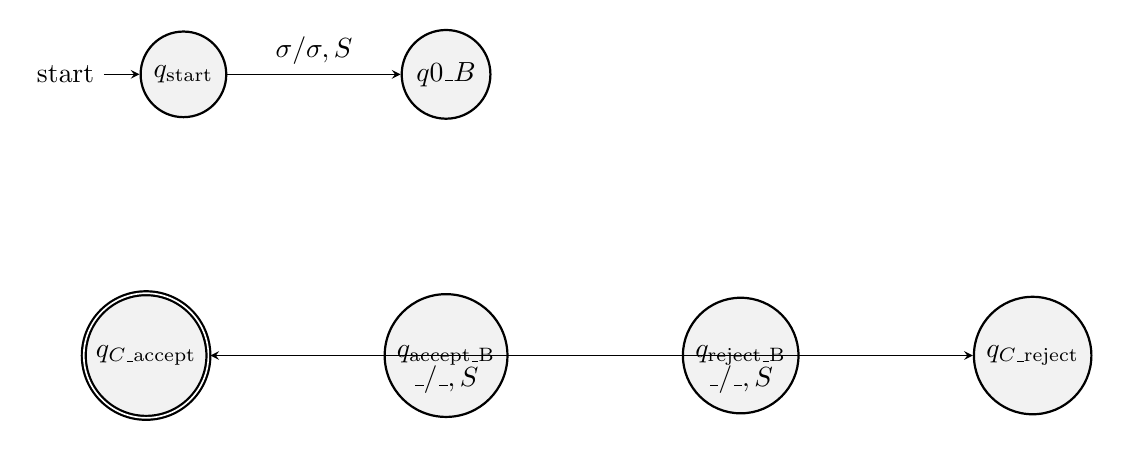
\begin{tikzpicture}

\node[state, initial] (qs) {$q_{\text{start}}$};
\node[state] (q0) [right=of qs] {$q0\_B$};
\node[state] (qaB) [below=of q0] {$q_{\text{accept\_B}}$};
\node[state] (qrB) [right=of qaB] {$q_{\text{reject\_B}}$};
\node[state, accepting] (qaC) [left=of qaB] {$q_{C\_\text{accept}}$};
\node[state] (qrC) [right=of qrB] {$q_{C\_\text{reject}}$};

\draw (qs) edge[above] node{$\sigma / \sigma , S$} (q0);

\draw (qaB) edge[below] node{$\_ / \_ , S$} (qrC);
\draw (qrB) edge[below] node{$\_ / \_ , S$} (qaC);

\end{tikzpicture}
\end{center}

\section{Conclusão}

As três Máquinas de Turing aqui apresentadas formam um conjunto completo para demonstrar técnicas de:
\begin{itemize}
    \item balanceamento por marcação (A)
    \item contagem relacional por marcação múltipla (B)
    \item complemento por inversão de estados finais (C)
\end{itemize}

\end{document}